\documentclass[10pt,xcolor={dvipsnames}, aspectratio=169]{beamer}
\usetheme[
%%% option passed to the outer theme
%    progressstyle=fixedCircCnt,   % fixedCircCnt, movingCircCnt (moving is deault)
  ]{Feather}
  
% If you want to change the colors of the various elements in the theme, edit and uncomment the following lines

% Change the bar colors:
\setbeamercolor{Feather}{fg=NavyBlue!20,bg=NavyBlue}

% Change the color of the structural elements:
\setbeamercolor{structure}{fg=NavyBlue}

% Change the frame title text color:
\setbeamercolor{frametitle}{fg=black!5}

% Change the normal text colors:
\setbeamercolor{normal text}{fg=black!75,bg=gray!5}

%% Change the block title colors
\setbeamercolor{block title}{use=Feather,bg=Feather.fg, fg=black!90} 


% Change the logo in the upper right circle:
%\renewcommand{\logofile}{example-grid-100x100pt} 
%% This is an image that comes with the LaTeX installation
% Adjust scale of the logo w.r.t. the circle; default is 0.875
% \renewcommand{\logoscale}{0.55}

% Change the background image on the title and final page.
% It stretches to fill the entire frame!
% \renewcommand{\backgroundfile}{example-grid-100x100pt}

%-------------------------------------------------------
% INCLUDE PACKAGES
%-------------------------------------------------------

\usepackage[utf8]{inputenc}
\usepackage[utf8]{vietnam}
\usepackage[english]{babel}
\usepackage[T1]{fontenc}
\usepackage{amsmath}
\usepackage{algorithm,algorithmic}
% \usepackage{helvet}

%% Load different font packages to use different fonts
%% e.g. using Linux Libertine, Linux Biolinum and Inconsolata
% \usepackage{libertine}
% \usepackage{zi4}

%% e.g. using Carlito and Caladea
\usepackage{carlito}
\usepackage{caladea}
\usepackage{zi4}

%% e.g. using Venturis ADF Serif and Sans
% \usepackage{venturis}

%-------------------------------------------------------
% DEFFINING AND REDEFINING COMMANDS
%-------------------------------------------------------

% colored hyperlinks
\newcommand{\chref}[2]{
  \href{#1}{{\usebeamercolor[bg]{Feather}#2}}
}

%-------------------------------------------------------
% INFORMATION IN THE TITLE PAGE
%-------------------------------------------------------

\title[] % [] is optional - is placed on the bottom of the sidebar on every slide
{ % is placed on the title page
      \textbf{Task Scheduling In Real-time System}
}

\subtitle[Task Scheduling Algorithm Selection]
{
      \textbf{}
}

\author[Quang Khanh]
{      Quang Khanh \\
      {\ttfamily khanh.tq170083@gmail.com}
}

\institute[]
{%
      Hanoi University of Science and Technology\\
	  School of Information and Communication Technology
}

\date{\today}

%-------------------------------------------------------
% THE BODY OF THE PRESENTATION
%-------------------------------------------------------

\AtBeginSection[]
{
    \begin{frame}
        \frametitle{Table of Contents}
        \tableofcontents[currentsection]
    \end{frame}
}
\begin{document}

%-------------------------------------------------------
% THE TITLEPAGE
%-------------------------------------------------------

{\1% % this is the name of the PDF file for the background
\begin{frame}[plain,noframenumbering] % the plain option removes the header from the title page, noframenumbering removes the numbering of this frame only
  \titlepage % call the title page information from above
\end{frame}}


\begin{frame}{Content}{}
\tableofcontents
\end{frame}

\section{System overview}

\begin{frame}
{Google's Borg System} 
	

		\begin{columns}[T] % align columns
			\begin{column}{.48\textwidth}
			\begin{block}
			{\textbf{Google's Borg system is a cluster manager} that runs millions of jobs, from many thousands 
			of different applications, across a number of clusters each with up to ten thousands of machines}
			\end{block}
			\begin{block}
			{\textbf{Borg cell} is a set of machines grouped together} 
			\end{block}
		\end{column}%
		\hfill%
		\begin{column}{.48\textwidth}
			\begin{figure}
				\centering
				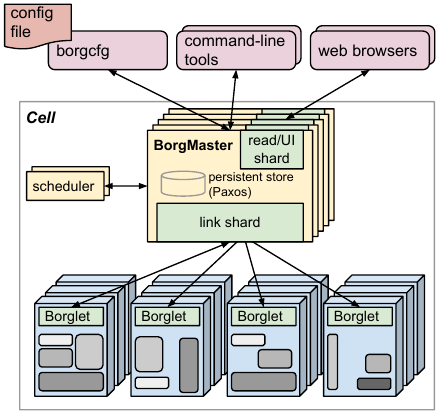
\includegraphics[scale=0.5]{images/borg_architecture.png}
				\caption{Borg architecture}
			\end{figure}
		\end{column}%
	\end{columns}
\end{frame}

\begin{frame}
{Google's Borg System} 
		\begin{columns}[T] % align columns
			\begin{column}{.48\textwidth}
			\begin{block}
			{\textbf{BorgMaster} is a logically centralized controller over a borg cell}
			\end{block}
			\begin{block}
			{\textbf{Borglet} is an agent process that runs on each machine in a cell}
			\end{block}
		\end{column}%
		\hfill%
		\begin{column}{.48\textwidth}
			\begin{figure}
				\centering
				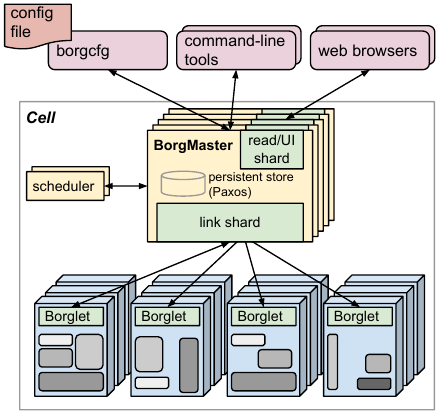
\includegraphics[scale=0.5]{images/borg_architecture.png}
				\caption{Borg architecture}
			\end{figure}
		\end{column}%
	\end{columns}
\end{frame}

\begin{frame}
{Task scheduling in Borg system}
		\begin{columns}[T] % align columns
			\begin{column}{.48\textwidth}
			\begin{block}
			{When a job is submitted}
			It is added to pending queue
			\end{block}
			\begin{block}
			{Scheduler}
			Scheduler scans the pending queue and assigns tasks to machines by scheduling algorithm. 
			The algorithm has two parts: 
			\begin{itemize}
				\item \textbf{feasiable checking: } to find machines on which the task could run
				\item \textbf{scoring: } to pick one machine to assign task to.
			\end{itemize}
			\end{block}
		\end{column}%
		\hfill%
		\begin{column}{.48\textwidth}
			\begin{figure}
				\centering
				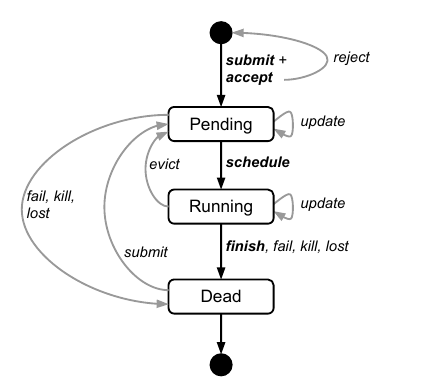
\includegraphics[scale=0.5]{images/task_states.png}
				\caption{Borg architecture}
			\end{figure}
		\end{column}%
	\end{columns}
\end{frame}

\begin{frame}
{Task scheduling algorithm in Borg system}
	\begin{block}
	{Feasible checking}
	The scheduler find a set of machines that: 
		\begin{itemize}
			\item meet the task's constraints (dependencies, packages, ...)
			\item have enough available resources
		\end{itemize}
	\end{block}
	
	\begin{block}
	{Scoring}
		The score is based on some criteria such as minimizing the number and priority of preempted tasks, and resources-related criteria are: 
		\begin{itemize}
			\item \textbf{worst fit}: speading workload across all the machines uniformly
			\item \textbf{best fit}: tries to fill machines as tightly as possible
		\end{itemize}
	\end{block}
\end{frame}

\section{Problem Statement}

\begin{frame}
{Drawbacks} 

	\begin{block}
	{Execution time} 
	Due to lack of certainty about how long the tasks' instructions are, the scheduler cannot estimate execution time of the tasks
	\end{block}
	
	\begin{block}
	{Service quanlity} 
	The solution cannot optimize execution time, leading to longer waiting-time to user	
	\end{block}
\end{frame}

\begin{frame}
{Drawbacks} 
	
	\begin{block}
	{Eviction}
	When resources of machines are not available, some running tasks would be evicted to release resources for higher-prioirty tasks
	\end{block}
	
	\begin{block}
	{Service quanlity}
	The user will have to wait longer to finish their job
	\end{block}
	
	\begin{block}
	{System effectiveness}
	The resources spent for the evicted tasks would be wasted. The google trace data published in 2011 shows that 
	up to 60\% of CPU resource is wasted by tasks that do not complete successfully.
	\end{block}
\end{frame}

\section{Solution}

\begin{frame}
{Length Estimation}
	\begin{block}
	{Divide tasks to two types:} 
		\begin{itemize}
			\item Long-running: the task as an always running service, unspecified its instructions
			\item Batch-job (short-running): the task which has specific instructions depending on only its input, which takes 
			from a few seconds to a few days to complete.
		\end{itemize}
	\end{block}
	
	\begin{block}
	{Long-running tasks}
	Find feasible machines and pick one of them for the task 
	\end{block}
	\begin{block}
	{Short-running tasks}
	Predict the intructions and find a machine in which the execution time is minimized
	\end{block}
\end{frame}

\begin{frame}
{Proposed task scheduling pipeline}
	\begin{figure}
		\centering
		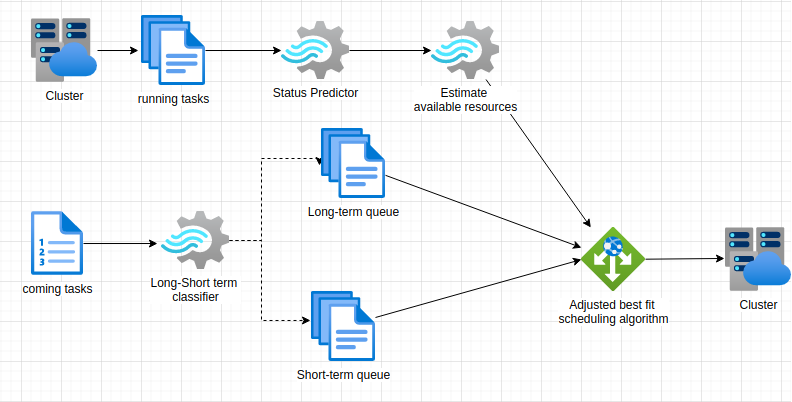
\includegraphics[scale=0.5]{images/scheduling_pipeline.png}
		\caption{Task scheduling pipeline}
	\end{figure}
\end{frame}

\begin{frame}
{Long-short term classifier} 
	\begin{columns}[T] % align columns
		\begin{column}{.48\textwidth}
			\begin{block}
			{Prior-knowledge classifier} 
			Basing on what kind of applications submitting tasks
			\end{block}
			\begin{block}
			{Logistic Classifier} 
			A logistic regression model to predict label of tasks
			\end{block}				
		\end{column}%
		\hfill%
		\begin{column}{.48\textwidth}
			\begin{figure}
				\centering
				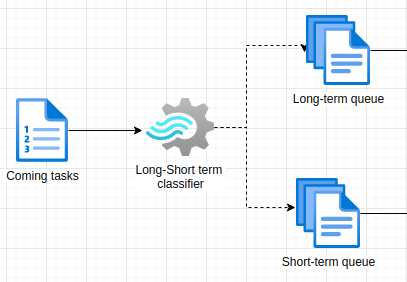
\includegraphics[scale=0.5]{images/long_short_classifier.png}
				\caption{Long-short term classifier}
			\end{figure}
		\end{column}%
	\end{columns}
\end{frame}

\begin{frame}
{Long-term task scheduling} 
	\begin{figure}
		\centering
		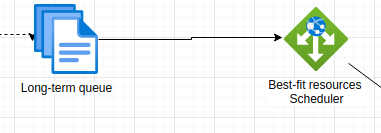
\includegraphics[scale=0.5]{images/long_term_queue.png}
		\caption{Long term task scheduling}
	\end{figure}
	\begin{block}
	{We should schedule long-term tasks first because in reality, they are always belonged to sensitive jobs such as Gmail, Docs in google trace data}
	\end{block}
	\begin{block}
	{Scheduling algorithm}
		\begin{itemize}
			\item Best fit: Optimize resources utilization
			\item Worst fit: Optimize time execution and workload balancing 
		\end{itemize}
	\end{block}
\end{frame}

\begin{frame}
{Proposed task scheduling pipeline}
	\begin{figure}
		\centering
		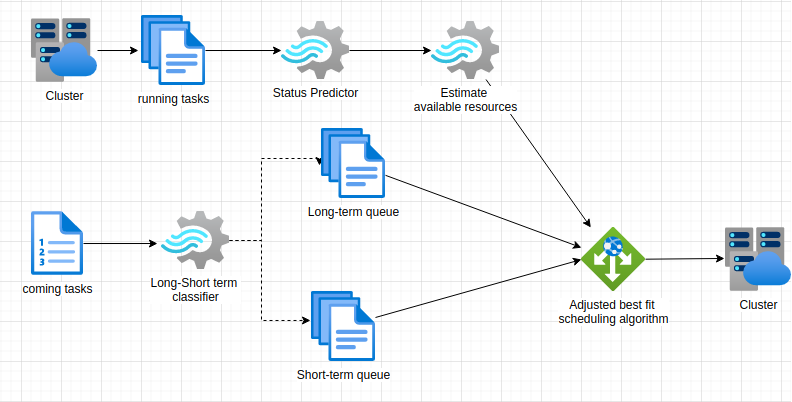
\includegraphics[scale=0.5]{images/scheduling_pipeline.png}
		\caption{Task scheduling pipeline}
	\end{figure}
\end{frame}


\begin{frame}
{Length predictor}
	\begin{figure}
		\centering
		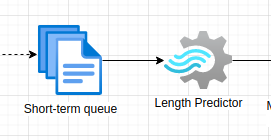
\includegraphics[scale=0.5]{images/length_predictor.png}
		\caption{Length predictor}
	\end{figure}
	\begin{block}
	{Task information}
		\begin{itemize}
			\item resources\_request
			\item meta\_data (priority, programming language, ...)
			\item length: the number of instructions 
		\end{itemize}
	\end{block}
	
	\begin{block}
	{Length estimation model}
	We expect that there is a machine learning model fitting task length data
	\end{block}
\end{frame}

\begin{frame}
{Minimizing execution time} 

	\begin{block}
	{Task execution time fomula}
		\begin{equation*}
			T = \frac{length}{MIPS * cpu\_usage}
		\end{equation*}
	\end{block}
	\begin{block}
	{Make-span}
		\begin{equation*}
			makespan = max(T_{1}, T_{2}, ..., T_{n})
		\end{equation*}
	\end{block}
	\begin{block}
	{Algorithm}
	\textbf{Input: }tasks, machines \\
	\textbf{Output: } task-machine mapping \\
	\textbf{Objective: } find a solution that minimize make-span of tasks
	\end{block}
\end{frame}

\begin{frame}
{Minimizing execution time algorithm}
	\begin{block}
	{Algorithm}
		\begin{algorithm}[H]
		\textbf{Input:} $L\_queue, S\_queue, vms$ \\ 
    	\textbf{Output:} Map<Task, Vm>
		\begin{algorithmic}[1]
			\STATE $usage \leftarrow \textbf{estimate\_usage}(vms)$
			\STATE $L\_running\_usage \leftarrow get\_L\_running(usage)$
			\STATE $S\_running\_usage \leftarrow get\_S\_running(usage)$
			\STATE $L\_solution \leftarrow \textbf{bestfit}(L\_queue, L\_running\_usage)$
			\STATE $L\_usage \leftarrow update(L\_running\_usage, L\_solution)$
			\STATE $S\_solution \leftarrow \textbf{bestfit}(S\_queue, S\_running\_usage)$
			\RETURN $merge(L\_solution, S\_solution)$
		\end{algorithmic}
		\caption{pseudocode for the calculation of }
		\label{alg:seq}
		\end{algorithm}
	\end{block}
\end{frame}

\begin{frame}
{Proposed task scheduling pipeline}
	\begin{figure}
		\centering
		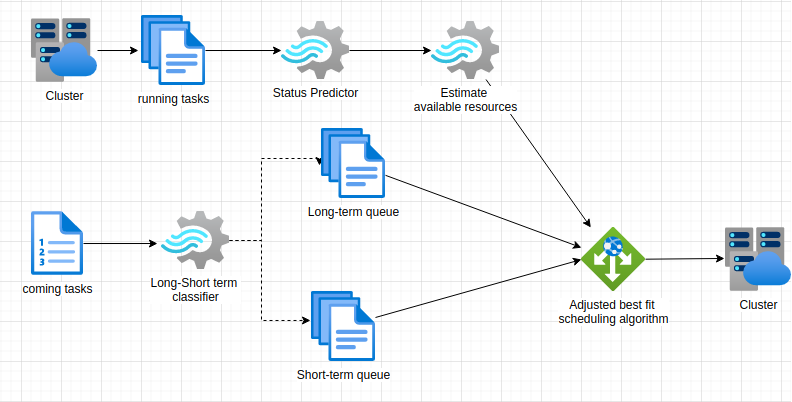
\includegraphics[scale=0.5]{images/scheduling_pipeline.png}
		\caption{Task scheduling pipeline}
	\end{figure}
\end{frame}


\begin{frame}
{Update long-short term}
	\begin{figure}
		\centering
		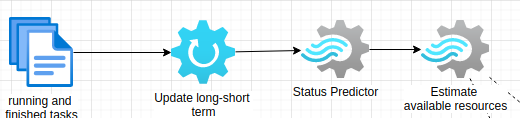
\includegraphics[scale=0.5]{images/status_estimation.png}
		\caption{Update long-short term}
	\end{figure}
	
	\begin{block}
	{When the duration of a short-term task is extremly longer than the expected, the task would be re-labled as long-term}
		\begin{equation*}
			T = \frac{length}{MIPS * cpu\_usage} + \epsilon
		\end{equation*}
	\end{block}
\end{frame}

\begin{frame}
{Update long-short term}
	\begin{columns}[T]
		
		\begin{column}{0.6\textwidth}
			\begin{block}
			{Task execution time} 
				\begin{equation*}
					T \sim \mathcal{N}(\mu,\,\sigma^{2}) = \frac{1}{\sqrt{2\pi}\sigma}e^{\frac{(T - \mu)^{2}}{2\sigma^{2}}}
				\end{equation*}
			\end{block}
			\begin{block}
			{Task's duration}
				\begin{align*}
					P(T > duration) &= \int_{duration}^{\infty} \frac{1}{\sqrt{2\pi}\sigma}e^{\frac{(t - \mu)^{2}}{2\sigma^{2}}} \,dt \\
									&= \frac{1}{2} - \phi(\frac{duration - \mu}{\sigma})
				\end{align*}
			\end{block}
			\begin{block}
			{$\alpha$ threshold}
			$P(T > duration) < \alpha \rightarrow$ task is re-labeled as long-term
			\end{block}	
		\end{column}
		
		\hfill
		
		\begin{column}{0.4\textwidth}
			\begin{figure}
				\centering
				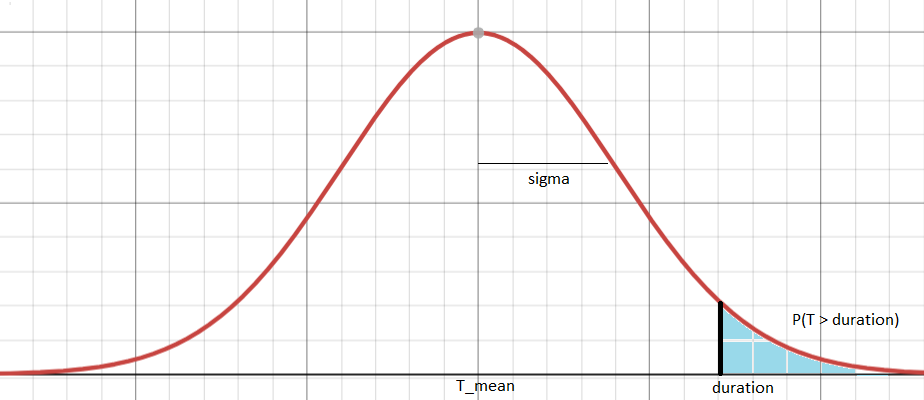
\includegraphics[scale=0.18]{images/duration_prob.png}
				\caption{Task execution time distribution}
			\end{figure}
		\end{column}		
			
	\end{columns}


\end{frame}

\begin{frame}
{Status predictor}
	\begin{columns}[T]
	
		\begin{column}{0.48\textwidth}
			\begin{block}
			{Uncertain state}
				\begin{itemize}
					\item tasks are scheduled over $state_{1}$
					\item tasks are executed over $state_{2}$
				\end{itemize}
			$state_{1}$ and $state_{2}$ are probably biased.
			\end{block}
			
			\begin{block}
			{Estimate $state_{2}$}
			Basing on $state_{1}$, we want to estimate $state_{2}$ in order to get more accuracy environment information
			\end{block}
		\end{column}

		\hfill		
		
		\begin{column}{0.48\textwidth}
			\begin{figure}
				\centering
				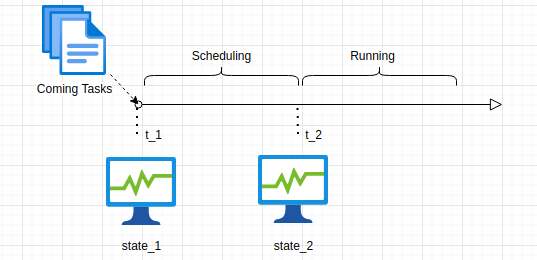
\includegraphics[scale=0.4]{images/state_change.png}
				\caption{Scheduling process}
			\end{figure}		
		\end{column}
	\end{columns}
	
\end{frame}

\begin{frame}
{Status predictor}
	\begin{columns}[T]
	
		\begin{column}{0.48\textwidth}
			\begin{block}
			{Task state}
				\textbf{Idea: } use Markov chain to estimate transition probabilities between the states
			\end{block}
			
			\begin{block}
			{Markov chain drawbacks}
			In experiment, the idea poses many problems :
				\begin{itemize}
					\item transition probabilities also depend on the duration of task
					\item cpu usage is also correlated to probability
				\end{itemize}
			\end{block}
		
		\end{column}

		\hfill		
		
		\begin{column}{0.48\textwidth}
			\begin{figure}
				\centering
				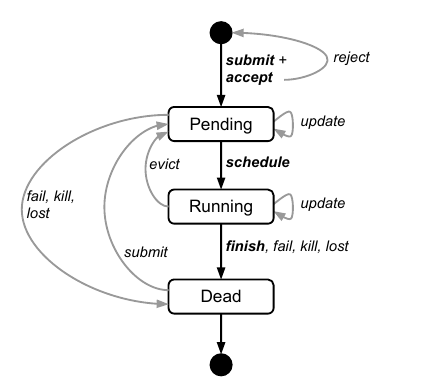
\includegraphics[scale=0.5]{images/task_states.png}
				\caption{Task states transition}
			\end{figure}		
		\end{column}
	\end{columns}

\end{frame}

\begin{frame}
{Status predictor}
	\begin{columns}[T]
	
		\begin{column}{0.5\textwidth}
			\begin{figure}
				\centering
				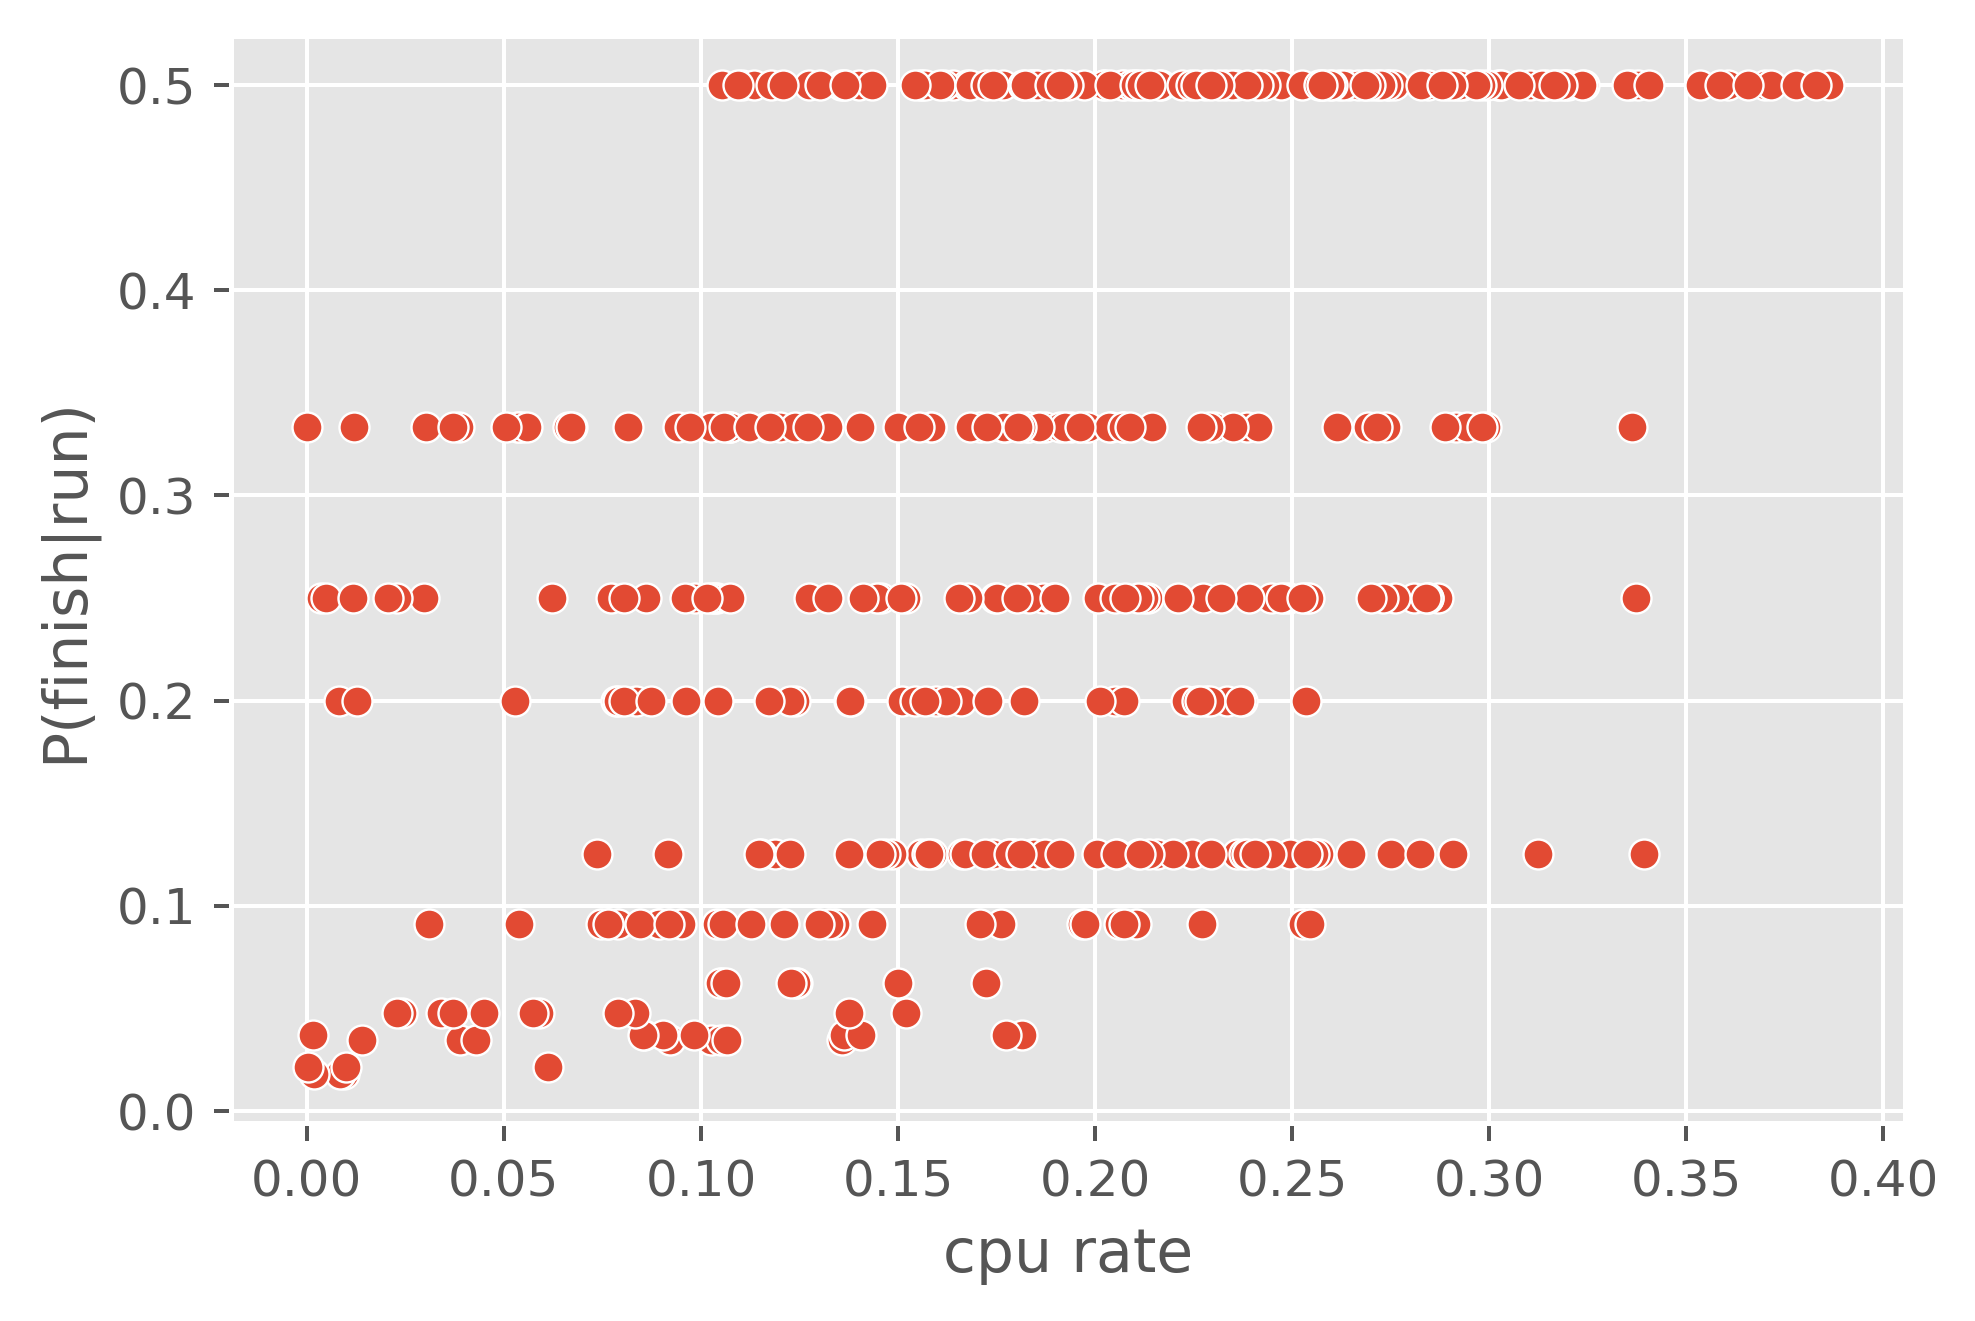
\includegraphics[scale=0.6, height=5cm]{images/cpu_vs_pro_img.png}
				\caption{cpuRequest vs transition probability}
			\end{figure}
		\end{column}

		\hfill		
		
		\begin{column}{0.48\textwidth}
			\begin{figure}
				\centering
				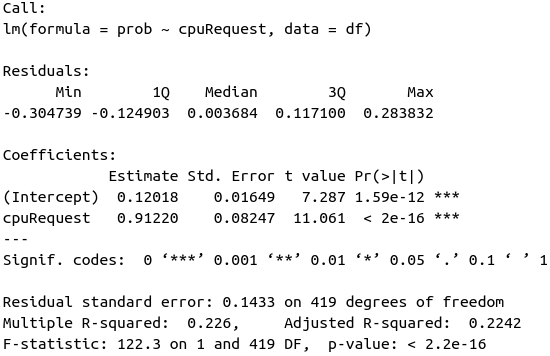
\includegraphics[height=5cm, width=6cm]{images/cpu_vs_prob.png}
				\caption{Summary statistics}
			\end{figure}		
		\end{column}
	\end{columns}

\end{frame}

\begin{frame}
{Bayesian network predictor}
	\begin{columns}[T]
	
		\begin{column}{0.6\textwidth}
			\begin{block}
			{Bayesian network}
				\begin{equation*}
					P(S_{i+1}|T_{i+1}, cpu, S_{i}) = \mathcal{F}_{S_{i+1}}(S_{i}, T_{i+1}, cpu, \theta)
				\end{equation*}
			\end{block}
			
			\begin{block}
			{Probability function}
				\begin{equation*}
					\mathcal{A}_{S_{i+1}}(S, T, cpu, \theta) = \theta_{0}^{S_{i+1}} + \theta_{1}^{S_{i+1}}*S + \theta_{2}^{S_{i+1}}*T + \theta_{3}^{S_{i+1}}*cpu
				\end{equation*}
				
				\begin{equation*}
					\mathcal{F}_{S_{i+1}}(S_{i}, T_{i+1}, cpu, \theta) = \frac{\mathcal{A}_{S_{i+1}}(S, T, cpu, \theta)}{\sum_{S_{k} \in \{S\}}{\mathcal{A}_{S_{k}}(S, T, cpu, \theta)}}
				\end{equation*}
			\end{block}
		\end{column}

		\hfill		
		
		\begin{column}{0.4\textwidth}
			\begin{figure}
				\centering
				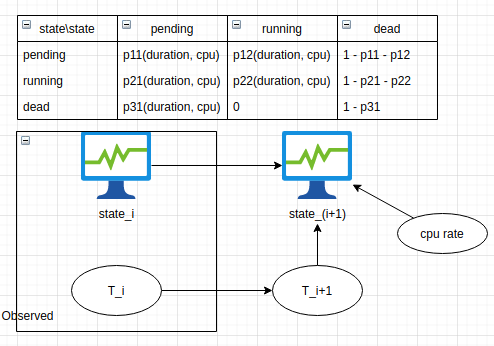
\includegraphics[height=5cm, width=6cm]{images/bayesian_predictor.png}
				\caption{Transition network}
			\end{figure}		
		\end{column}
	\end{columns}
\end{frame}

\begin{frame}
{Bayesian network predictor}
	\begin{columns}[T]
	
		\begin{column}{0.6\textwidth}
			\begin{block}
			{Probability factorization}
				\begin{align*}
					P(S_{i+1}|S_{i}, T_{i}, cpu) &= \int{P(S_{i + 1}, T_{i+1}|S_{i}, T_{i}, cpu)dT_{i+1}} \\
												&= \int{P(S_{i+1}|S_{i}, T_{i+1}, cpu)P(T_{i+1}|T_{i})dT_{i+1}} \\
												&= E_{T_{i+1} \sim \mathcal{N}(T_{i} + \mu, \sigma^{2})}\mathcal{F}_{S_{i}, cpu, \theta}(T_{i+1})\\
												&\sim \mathcal{F}_{S_{i}, cpu, \theta}(T_{i} + \mu)
				\end{align*}
			\end{block}
			
			\begin{block}
			{Use gradient ascend to find $\theta$ that maximize likelihood}
				\begin{equation*}
					\mathcal{L}(\theta: d) = log(\mathcal{F}_{S_{i}, cpu, \theta}(T_{i} + \mu))
				\end{equation*}
			\end{block}
		\end{column}

		\hfill		
		
		\begin{column}{0.4\textwidth}
			\begin{figure}
				\centering
				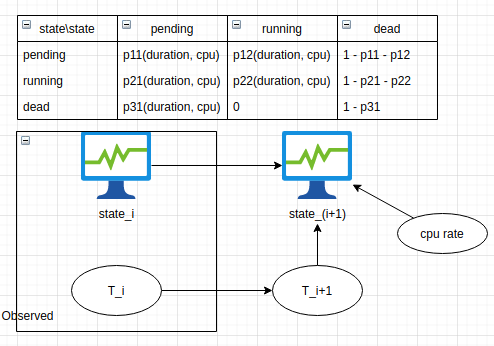
\includegraphics[height=5cm, width=6cm]{images/bayesian_predictor.png}
				\caption{Transition network}
			\end{figure}		
		\end{column}
	\end{columns}
\end{frame}

\begin{frame}
{Resources estimation}
	
	\begin{block}
	{Tasks assigned to machines}
		$\mathcal{S}$ is a set of tasks which are assigned to the machine and haven't finished
	\end{block}		
	
	\begin{block}
	{Resources usage estimation}
		\begin{equation*}
			resource\_usage = \sum_{task \in \mathcal{S}}{P(running) * resouce\_usage\_of\_task}
		\end{equation*}
		\begin{equation*}
			available\_resource = total\_capacity - resource\_usage
		\end{equation*}
		\begin{itemize}
			\item P(running): probability that the task continue running after scheduling time
		\end{itemize}
	\end{block}
	\begin{block}
	{Scheduling information}
		Coming tasks would be scheduled over resources estimation, not observed resources at scheduling time
	\end{block}
\end{frame}

\section{Experiment result}

\begin{frame}
{Cpu usage experiment} 
	\begin{columns}
		\begin{column}{0.48\textwidth}
			\begin{figure}
				\centering
				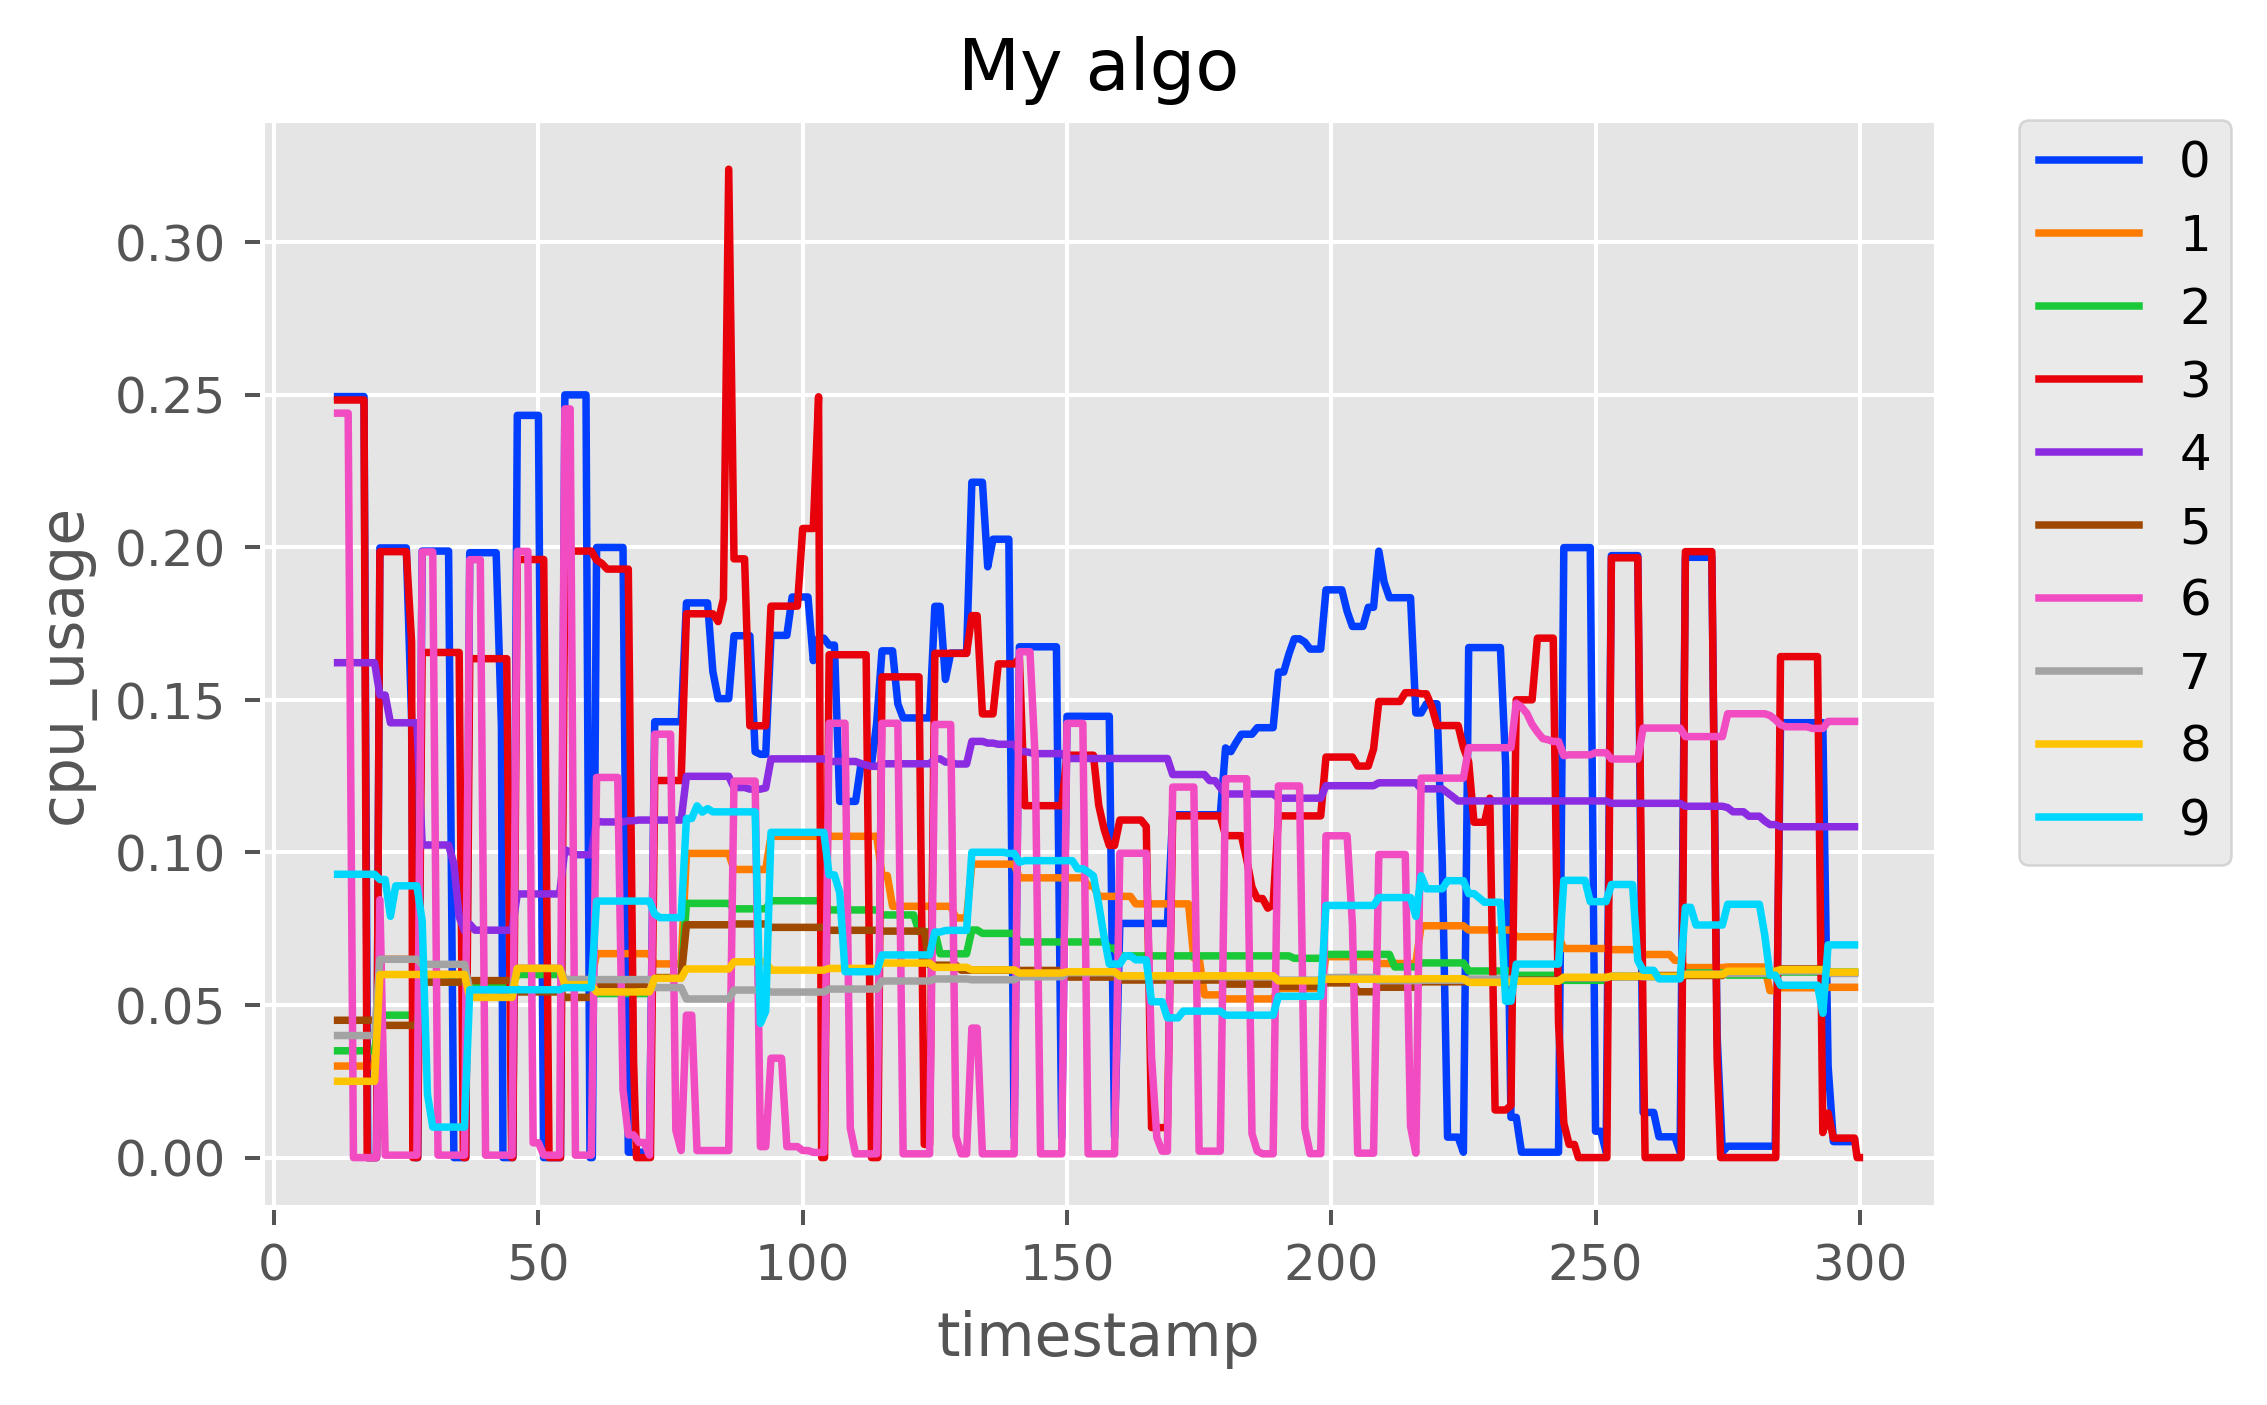
\includegraphics[scale=0.45]{images/myalgo_cpu.png}
			\end{figure}
		\end{column}

		\hfill		
		
		\begin{column}{0.48\textwidth}
			\begin{figure}
				\centering
				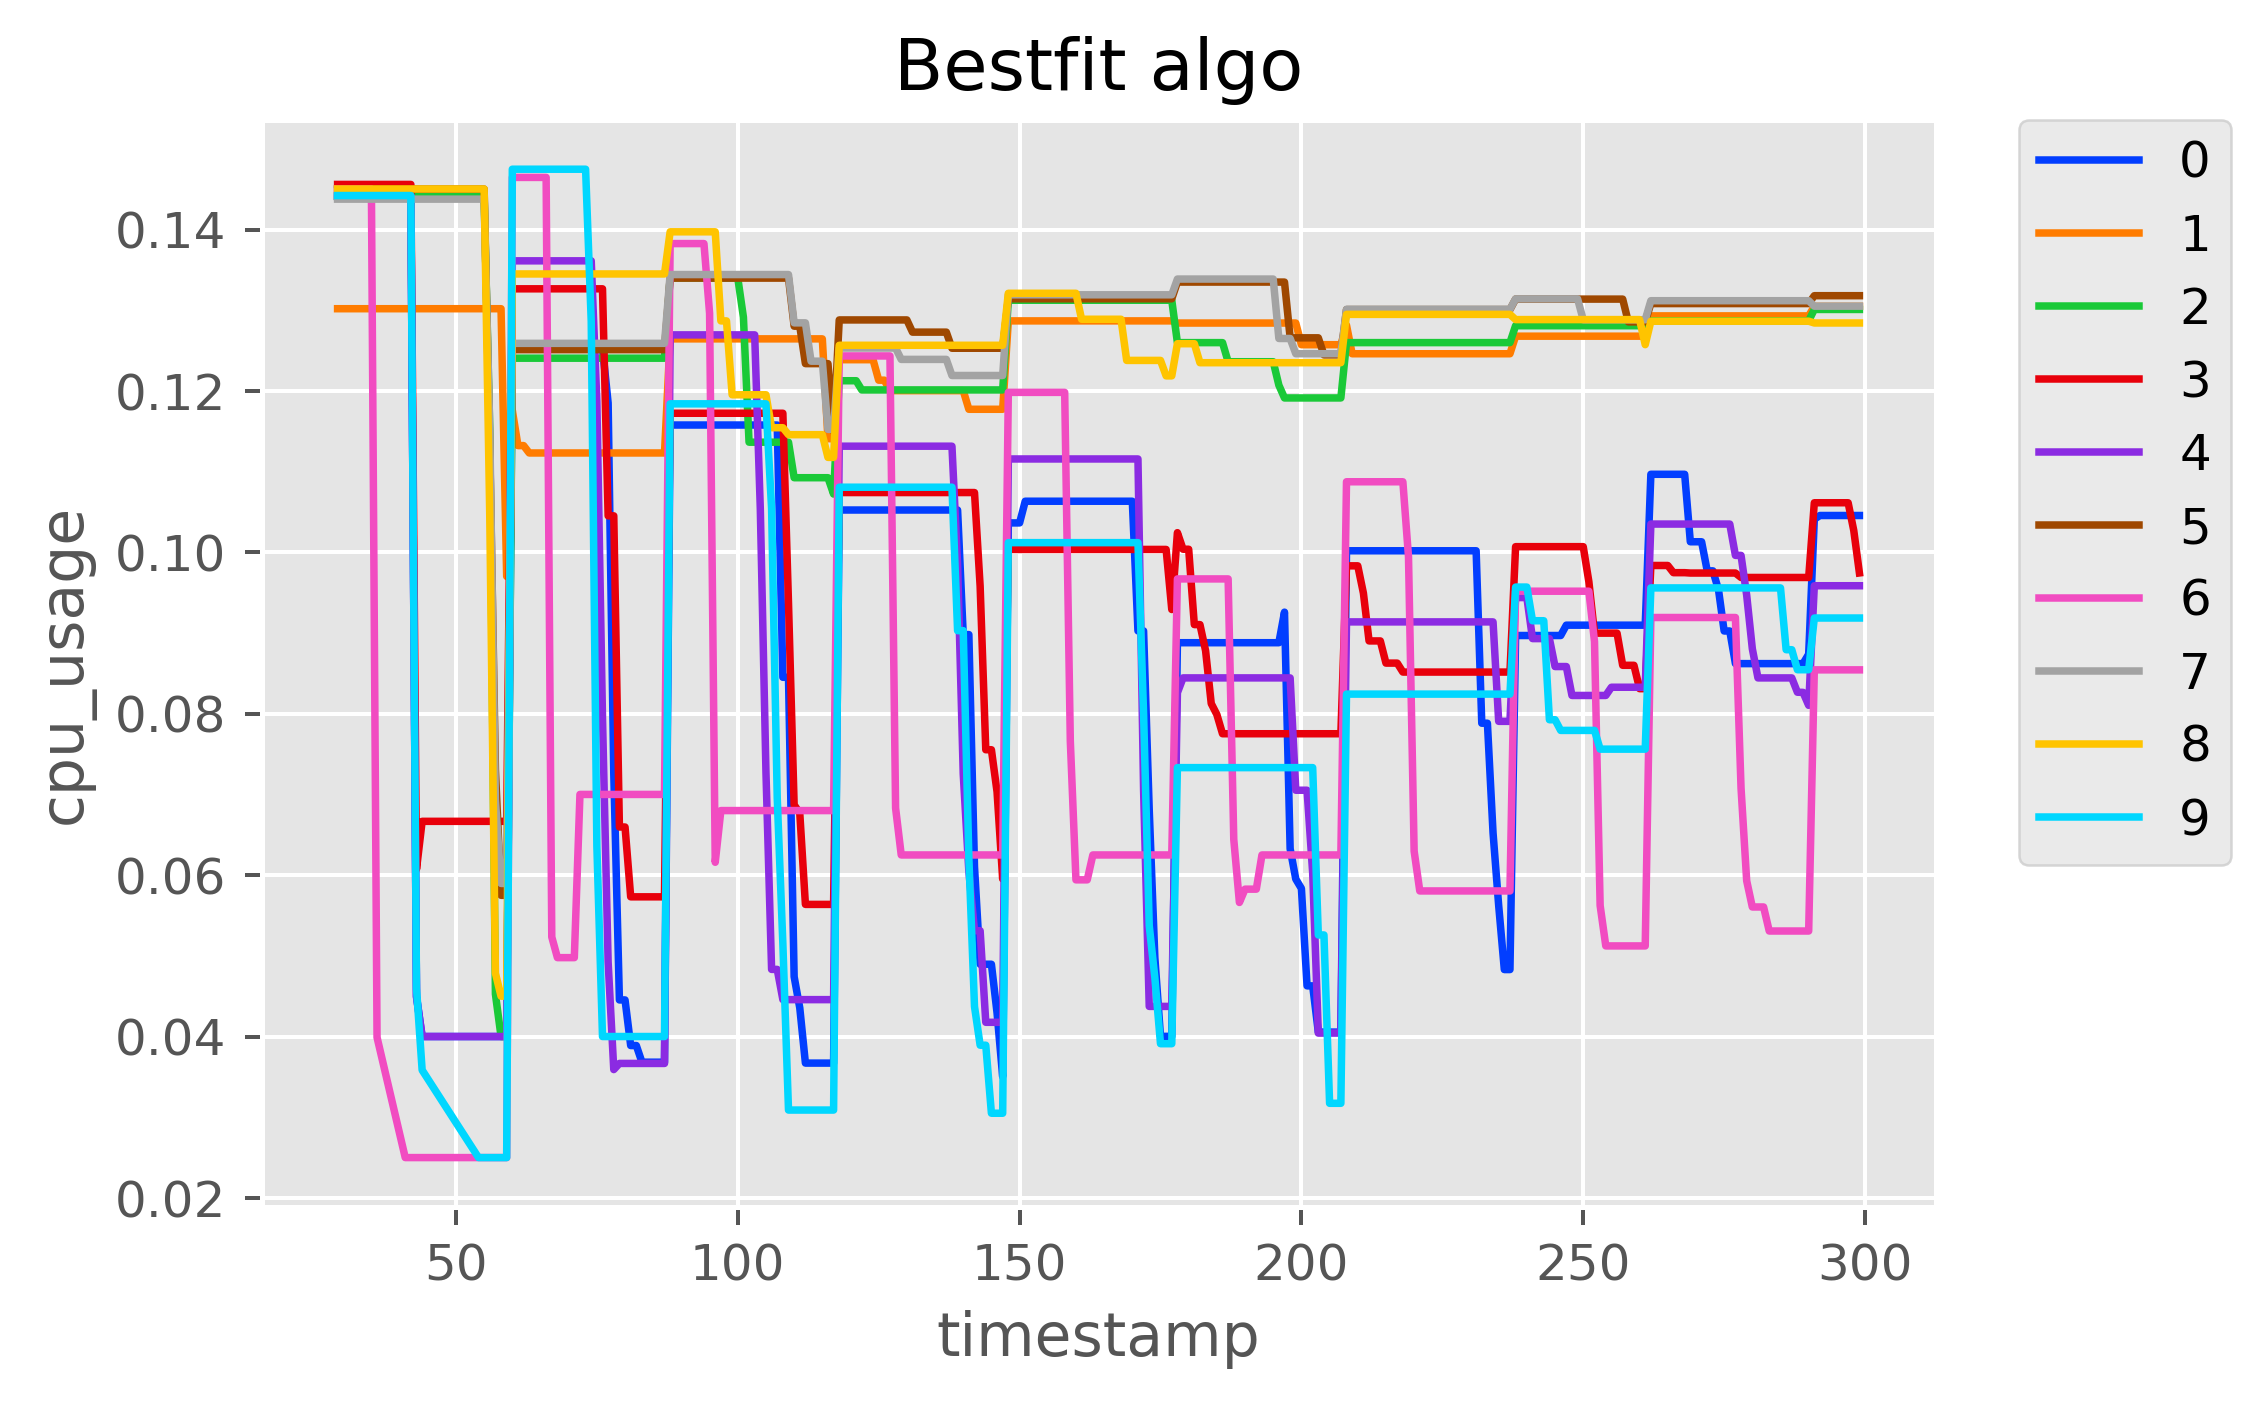
\includegraphics[scale=0.45]{images/bestfit_cpu.png}
			\end{figure}		
		\end{column}
	\end{columns}
\end{frame}

\begin{frame}
{Number of tasks finished}
	\begin{columns}
		\begin{column}{0.48\textwidth}
			\begin{figure}
				\centering
				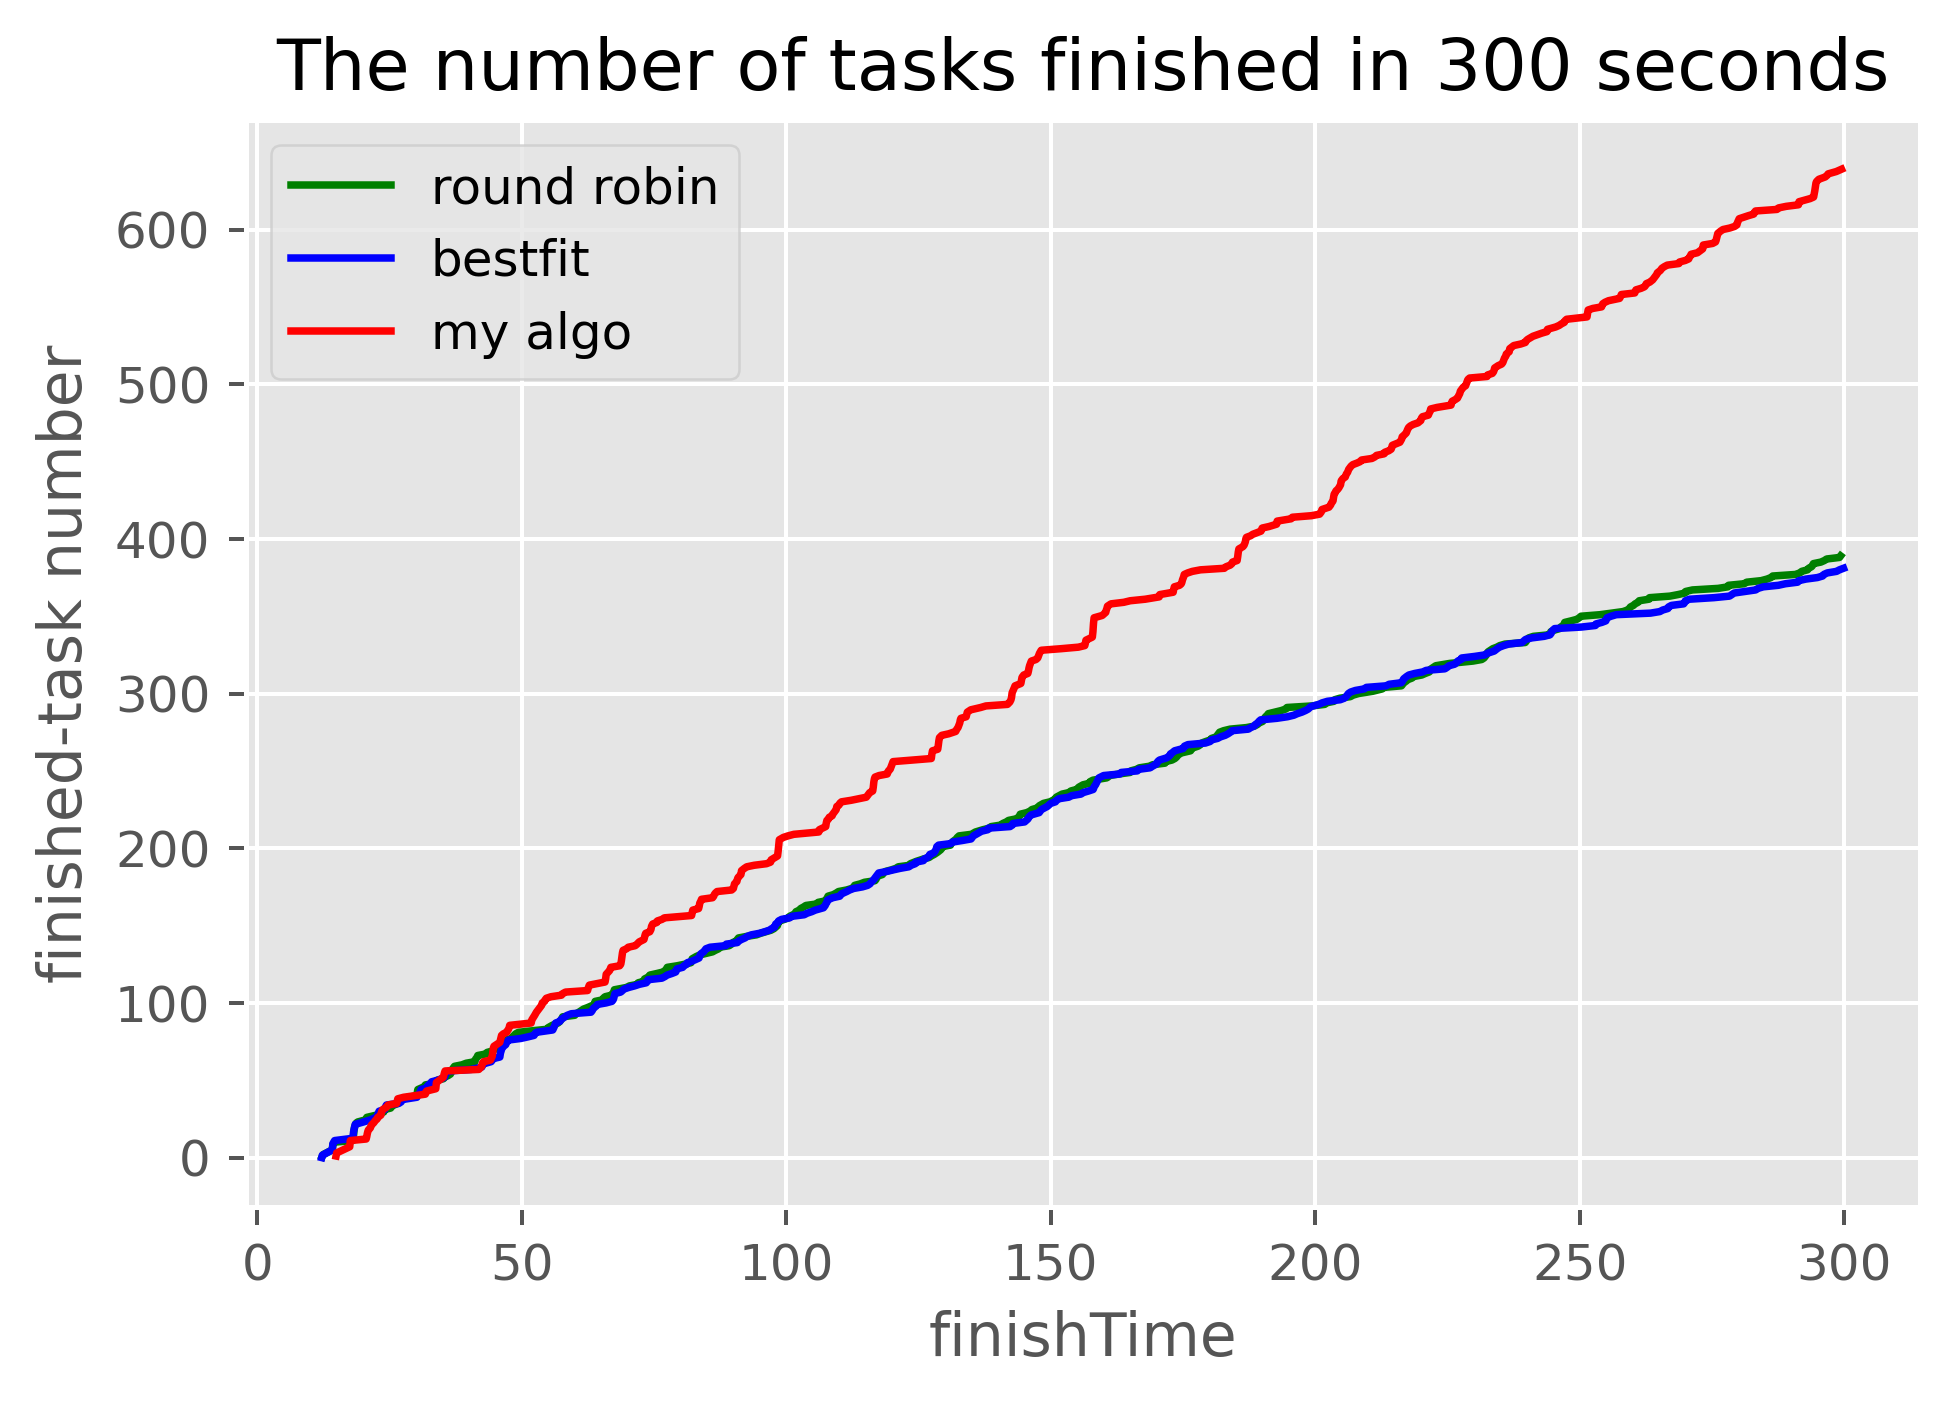
\includegraphics[scale=0.6, height=5cm]{images/tasks_accumulation.png}
			\end{figure}
		\end{column}

		\hfill		
		
		\begin{column}{0.48\textwidth}
			\begin{figure}
				\centering
				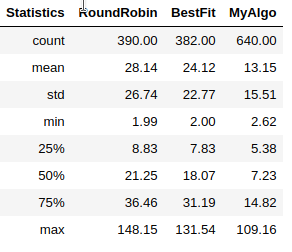
\includegraphics[scale=0.7, height=5cm]{images/running_statistics.png}
			\end{figure}		
		\end{column}
	\end{columns}
\end{frame}

\begin{frame}
{Resouces estimation}
	\begin{columns}
		\begin{column}{0.48\textwidth}
			\begin{figure}
				\centering
				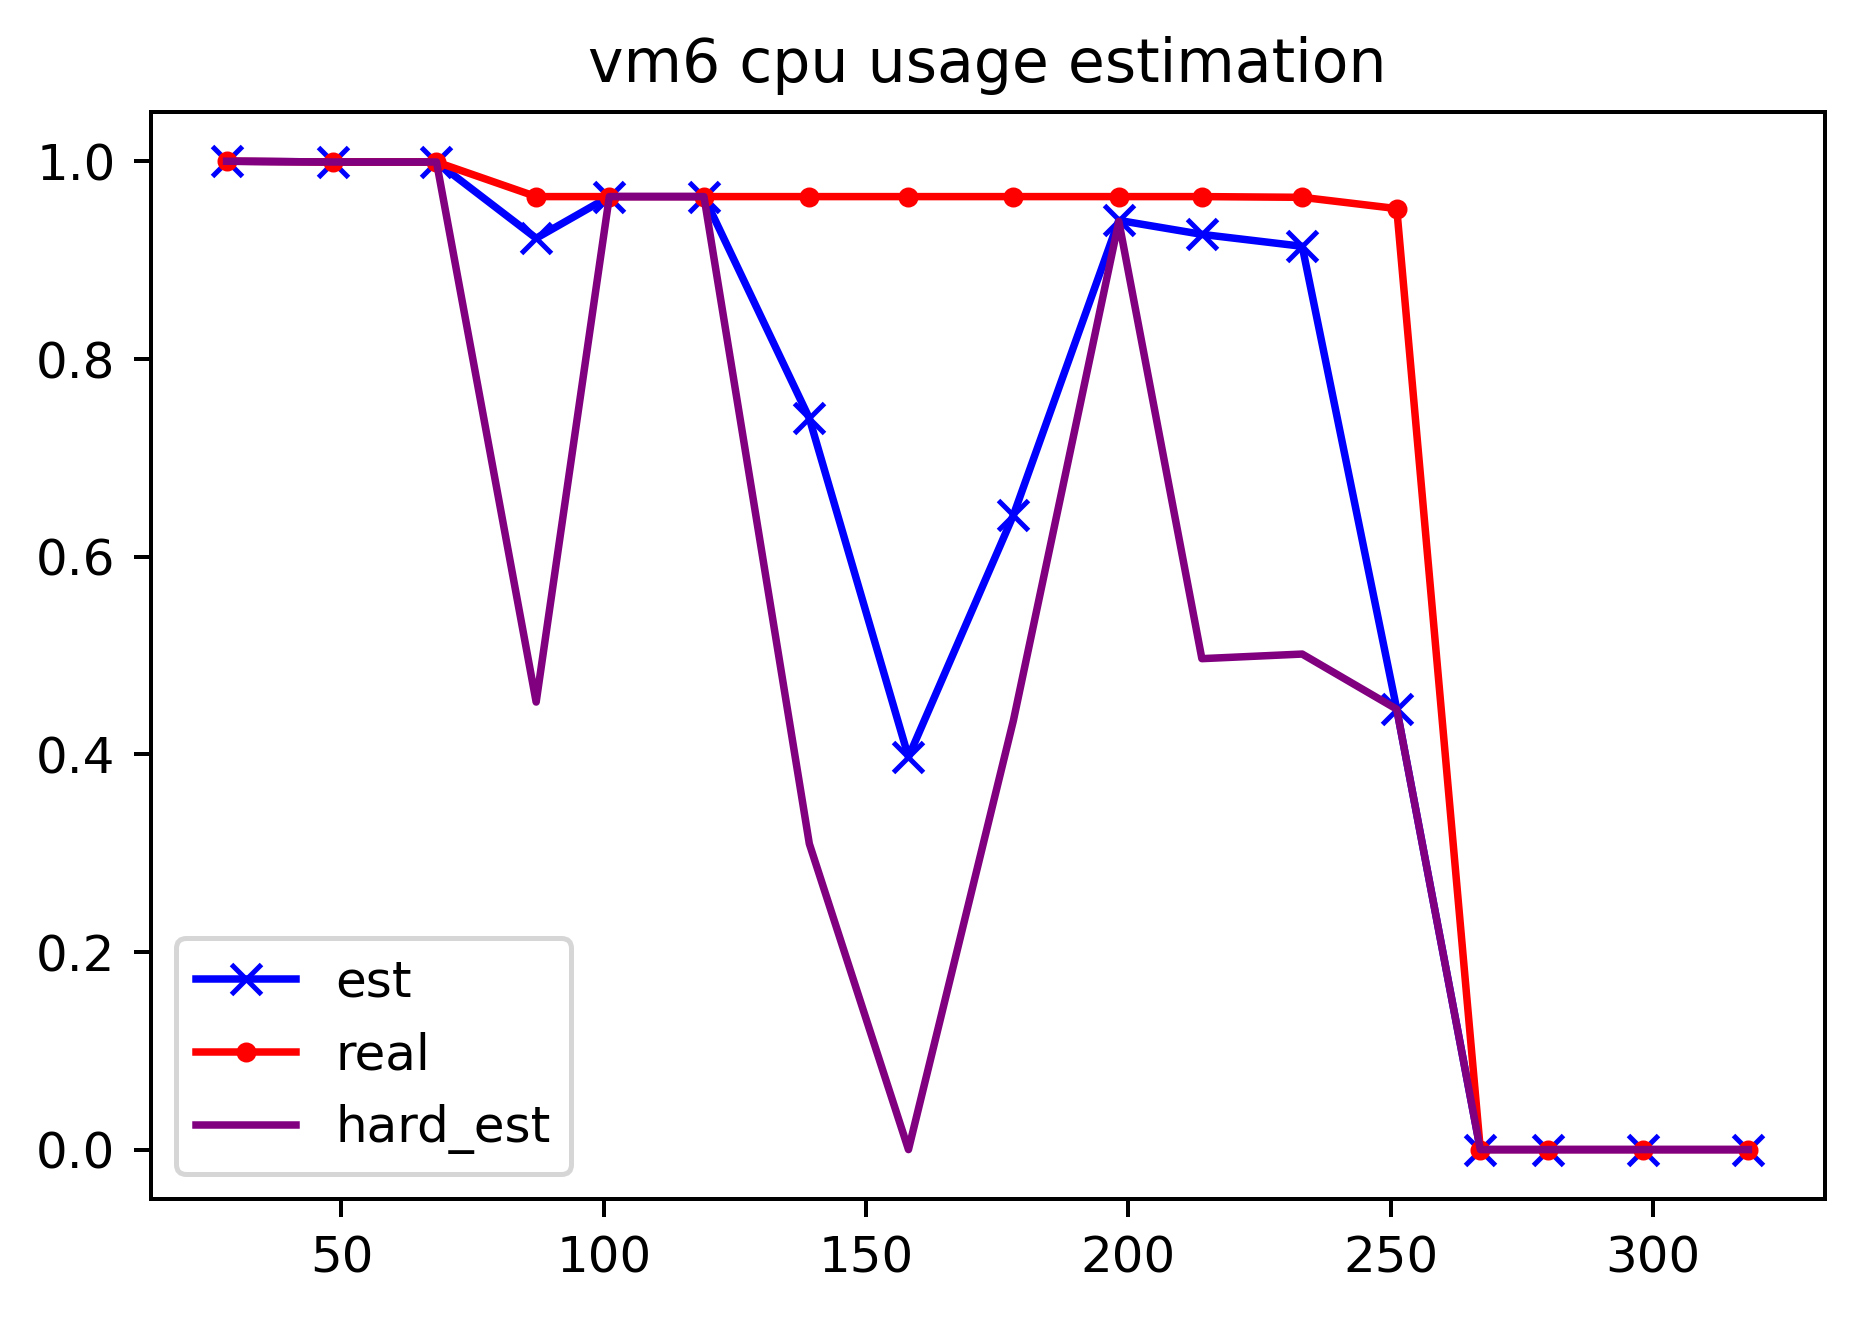
\includegraphics[scale=0.6, height=5cm]{images/cpu_usage_estimation_1.png}
			\end{figure}
		\end{column}

		\hfill		
		
		\begin{column}{0.48\textwidth}
			\begin{figure}
				\centering
				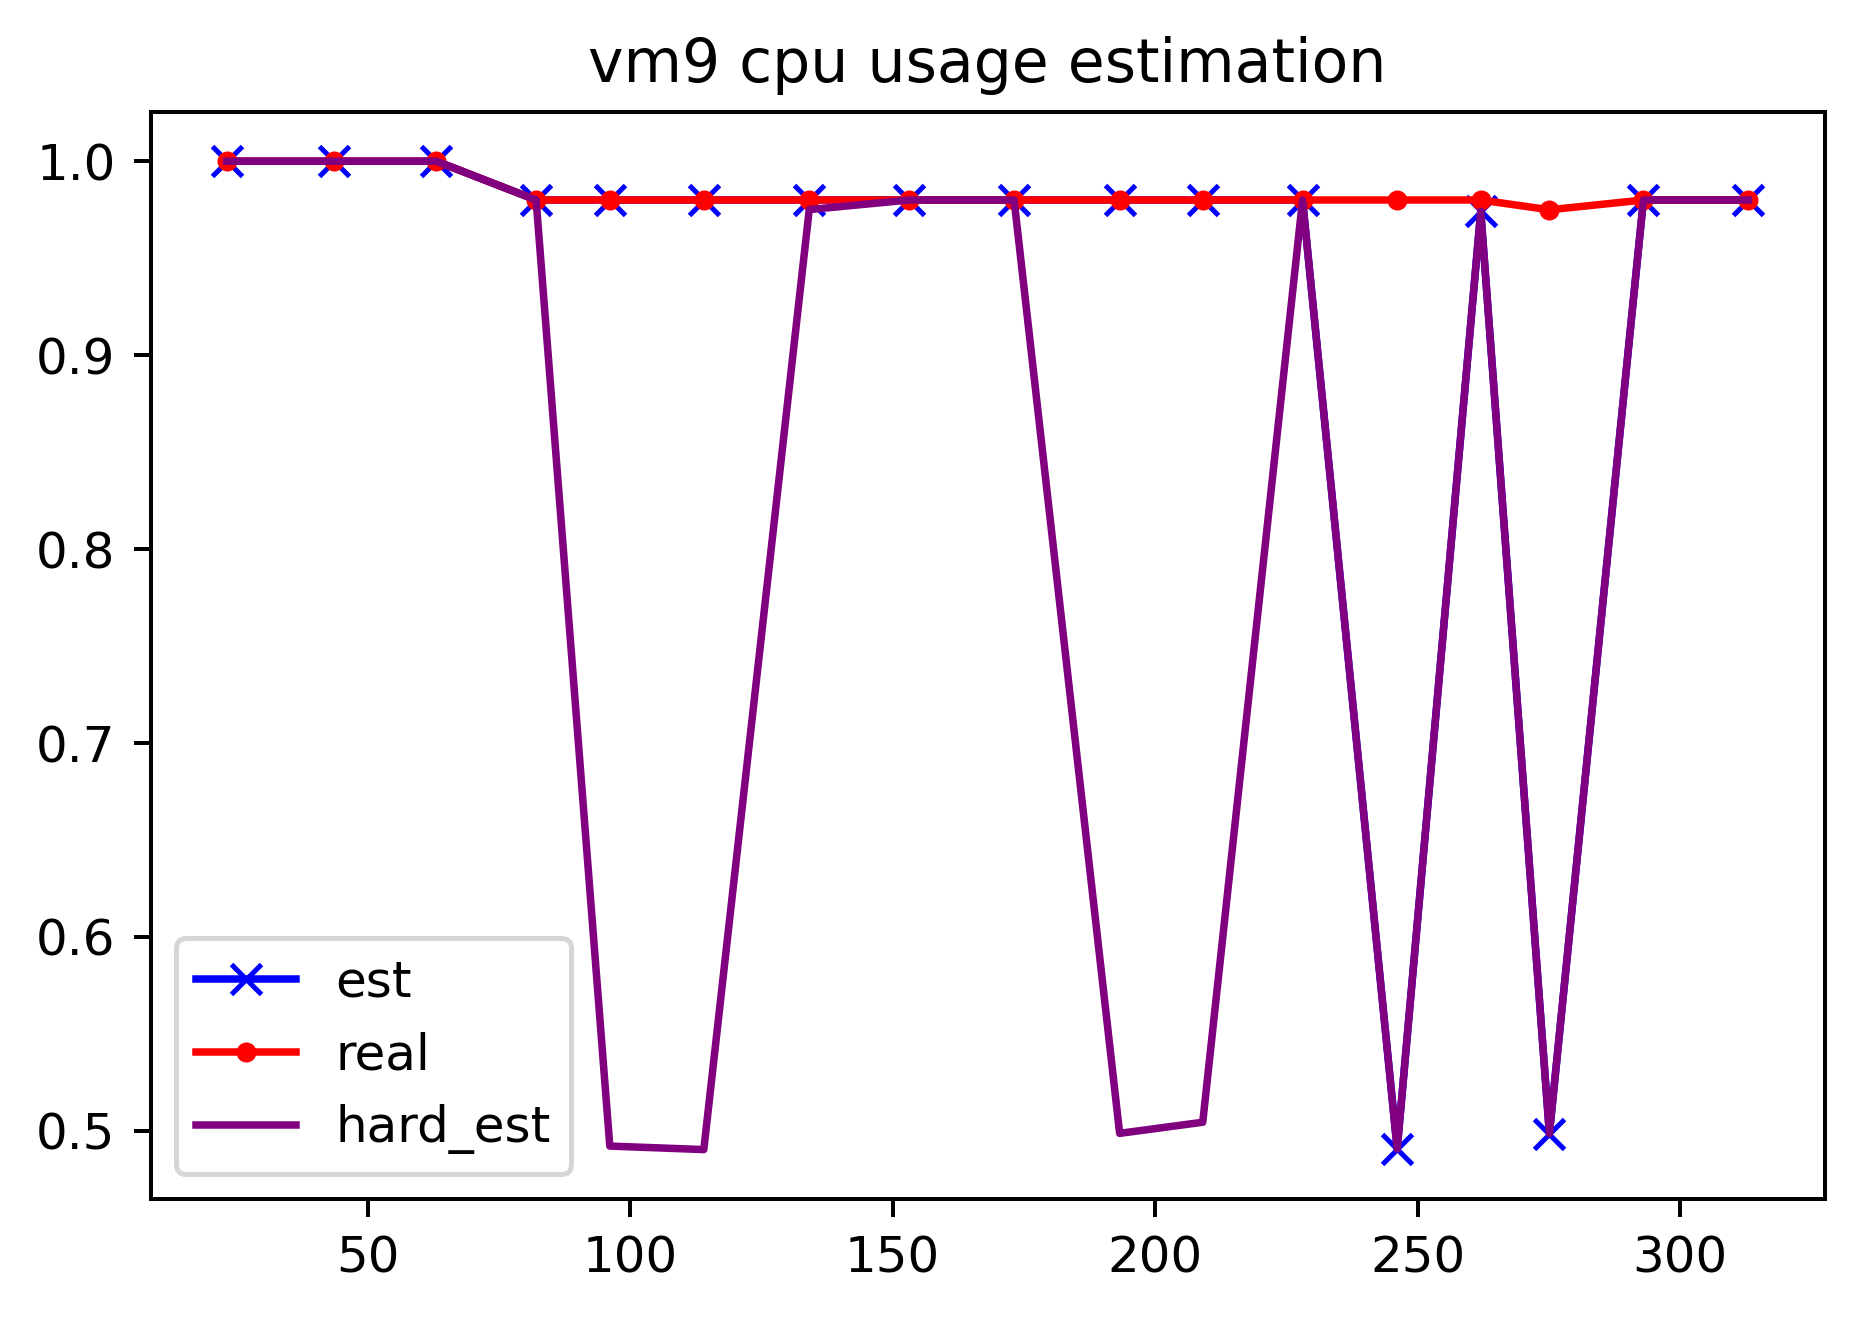
\includegraphics[scale=0.6, height=5cm]{images/cpu_usage_estimation_2.png}
			\end{figure}		
		\end{column}
	\end{columns}
\end{frame}

\begin{frame}
{Resources estimation}
	\begin{block}
	{Comparison between available-resouces estimation vs no estimation}
		\begin{figure}
			\centering
			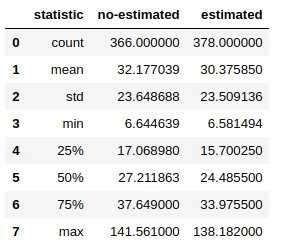
\includegraphics[scale=0.7]{images/estimate_comparison.png}
		\end{figure}
	\end{block}
\end{frame}


{\1
\begin{frame}[plain,noframenumbering]
  \finalpage{Thank you for listening!}
\end{frame}}

\end{document}